\chapter{Results}
\label{results}

\section{Dead projects}
\label{section:deads}
The data set of 250 projects contains data points up to June 2013, because the
data was gathered in July 2013.

The data set contains 21 (8.4\%) dead projects. A total of 38 (15.2\%) projects
complied to the definition of a dead project as defined in section
\ref{def:dead}, but manual verification of the 38 potential dead projects, with
data up to April 2014, revealed that 21 (8.4\%) are \emph{really }\rm dead.

For each of the 38 projects, the project's website, source code repository, and
commit history was consulted. The 21 dead projects and their $age\_in\_months$
at the moment of death as a result of the verification are shown in Table
\ref{table:deads}.

\begin{wraptable}{l}{40mm}
\caption{Dead projects}\label{table:deads}
\centering
\begin{tabular}{rr}
  \hline
 ID & Died at month \\ 
  \hline
317799 &   2 \\ 
  587198 &   3 \\ 
  588411 &   5 \\ 
  589515 &   7 \\ 
  587204 &   8 \\ 
  585077 &   9 \\ 
  587571 &  11 \\ 
  586805 &  14 \\ 
  360279 &  30 \\ 
  322065 &  37 \\ 
  11389 &  46 \\ 
  12053 &  68 \\ 
  3085 &  71 \\ 
  307140 &  71 \\ 
  4614 &  75 \\ 
  41745 &  80 \\ 
  155830 &  84 \\ 
  325178 &  92 \\ 
  4007 & 120 \\ 
  15700 & 121 \\ 
  12547 & 142 \\  
   \hline
\end{tabular}
\end{wraptable}

\paragraph{}
All, except one, of the projects in Table \ref{table:deads} are dead because it
was abandoned by the community of contributors. Except for project with ID
587204, which is still receiving updates, but at very slow and sporadic
intervals. However, since the updates do not involve code activity, it is
considered dead.

\paragraph{}
The first 7 projects have died before their first anniversary. The tail 14
projects died between 14 and 142 months of age.

\paragraph{}
When zooming in on the project with ID 317799, which is the youngest in this set
and died in its second month, it shows that this project has had a history of
the slightest change in its lines of code evolution. The project has had a total
number of 7 commits during the time it is being tracked by Ohloh (since
September 2011 up to now). A total of 4 contributors have worked on the project
since it was tracked. The most recent commit was done in October 2011.

\paragraph{}
Project with ID 12547 is the oldest. It died after 142 tracked months and has
had its most recent commits in February 2012. A total of 10 contributors have
worked on this project since May 2000.

\paragraph{}
The special case project, with ID 587204, is the only project that is not
abandoned by its (entire) community. The project has had 3 contributors over its
lifetime. One of them is still active every now and then. The most recent
commits were done in January 2014, the commits before that were in June 2012.
The commits involved updates in documentation, and the creation of a
configuration file for a continuous integration server. These commits do not
involve code changes.

The project died in July 2012, after 8 months since the first data point
tracked.

\paragraph{}
The other 17 projects complying to the definition of dead (section
\ref{def:dead}) appeared to be still alive. For 9 of the projects activity is
very low or rapidly decreasing; 5 projects were migrated to another source code
repository; and for 3 projects the activity is increasing after a long period of
no activity.

\paragraph{}
The 9 projects with very low or decreasing activity show signs of 'dying'. Their
community is slowly but surely abandoning the project as can be seen by a
decrease of 35\% to 55\% of contributors, and/or commits.

The 5 migrated projects for which the tracking information is not updated at
Ohloh are lost. The tracking is stopped from the moment the project is
migrated. The tracking and analysis can be recovered by updating the source
code locations at Ohloh, but for this study the project is out of sight.

The 3 projects that have had no activity in a year, but after that show little
increase of activity are more difficult to explain. Manual evaluation showed
that there exist similar projects outside the data set that eventually die, but
there are also similar projects that eventually got 'resurrected'.

\section{Sequences and patterns}
The wavelet transform and first analysis step resulted in 1,669,448 similar
sequences found in project's LOC\footnote{LOC: see section
\ref{section:signals}} signals. Almost all of these sequences (1,669,432
(99.999\%)) were found in scale/filter coefficients in 250 distinct projects.
A mere 16 sequences were found in wavelet/shift coefficients occurring in 15
distinct projects.

\paragraph{}
The detection of popular sequences found 16,049 patterns\footnote{Pattern:
see section \ref{def:pattern}}. The patterns consist only of sequences
of scale/filter coefficients. This was to be expected; the 16 similar sequences
in shift coefficients are not similar within the group of sequences of shift
coefficients. Additionally, the shift coefficients are incomparable to the
filter coefficients because it is a fundamentally different way of signal
transformation. Mixing both types of coefficients would ignore how the
coefficients were found and invalidate the patterns.

The patterns occurred at least 5 times and at most 1,512 times. On average, a
pattern occurs 104 times. A single pattern occurs in at least 1 and at most 204
projects (36 projects on average). The pattern length is between 4 and 19
coefficients (on average 6) across various decomposition levels. Patterns are
found at levels 3 to 7. The higher the level, the closer the level of detail of
wavelet is to the original signal.

12,643 (79\%) of the patterns appear in both dead and alive projects; 3,390
(21\%) of the patterns appear in alive projects only; and 16 (0.1\%) of the
patterns appear in dead projects only.

\subsection{Pattern evaluation}
\label{section:pattern_evaluation}
To be able to know what the patterns represent, the 16,049 patterns are
projected onto the original signal. This is done by finding the project the
pattern was first detected, and taking the pattern's level of decomposition and
starting point in the series of coefficients for its project.

As the set of values of level of decomposition, starting point in the series,
its length (i.e., number of coefficients), and the originating project is
unique for each pattern, it can be 're-projected' onto the signal of that
particular project. This gives the $age\_in\_months$ values the sequence starts
and ends in the project.

Knowing the start and end month of a sequence within a project, the values of
the original signal during the sequence are captured for further analysis.

\paragraph{}
The sequences have a wide range in what they represent. The maximum difference
of the LOC value is computed for each sequence by computing the difference
between every two values. The maximum of the list of differences is taken as
the maximum LOC difference. The patterns have maximum LOC differences between 0
(i.e., no change in LOC over the series) and 502,999. Figure
\ref{figure:pattern_loc_diff} shows the distribution of this number across the
patterns.

\begin{figure}[H]
\caption{Distribution of maximum LOC differences across
patterns}\label{figure:pattern_loc_diff}
\centering
	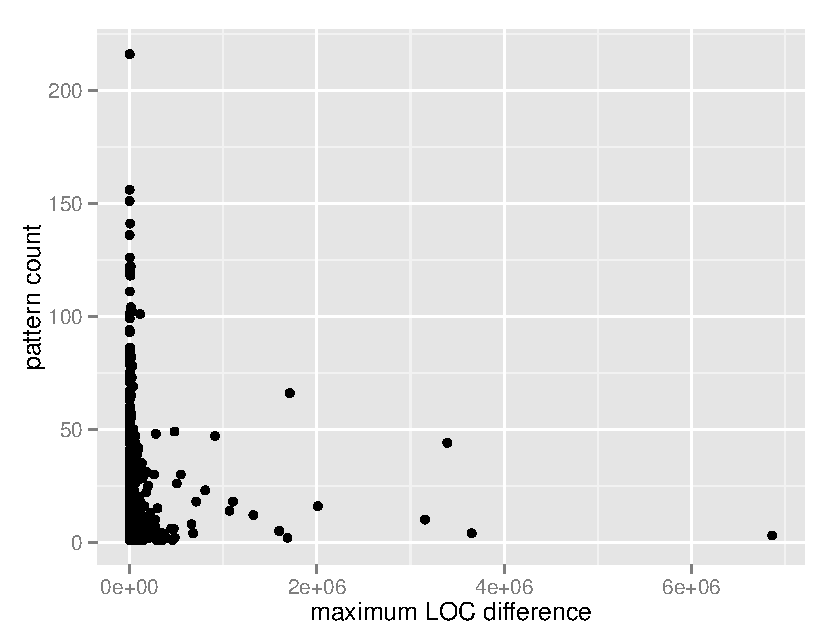
\includegraphics[width=296pt]{images/pattern_LOC_diff_100.pdf}
\end{figure}

75\% of the patterns have a maximum LOC difference less than 11,731; 50\% have a
maximum LOC difference less than 2,736; and 25\% less than 540. A maximum LOC
difference of 0 is the most common (5.22\%), followed by 3,994 (4.62\%), 9
(4.51\%), and 1,865 (3.11\%).

The above top four patterns with least maximum LOC differences are shown in
Figure \ref{figure:top_patterns_plots}. The figure illustrates the wavelets of
the patterns for all the project signals they were detected in, depicted as the
differences in LOC values between two subsequent coefficients.
The figure shows that the sequences have similar waveforms. Note that the
factor of scale is reintroduced, because the sequences all contain scale/filter
coefficients. The factor of time, however, is still being eliminated, hence the
use of index on the horizontal axis.

\begin{figure}[H]
\caption{The four most common type A patterns projected onto original
signal}\label{figure:top_patterns_plots}
\centering
	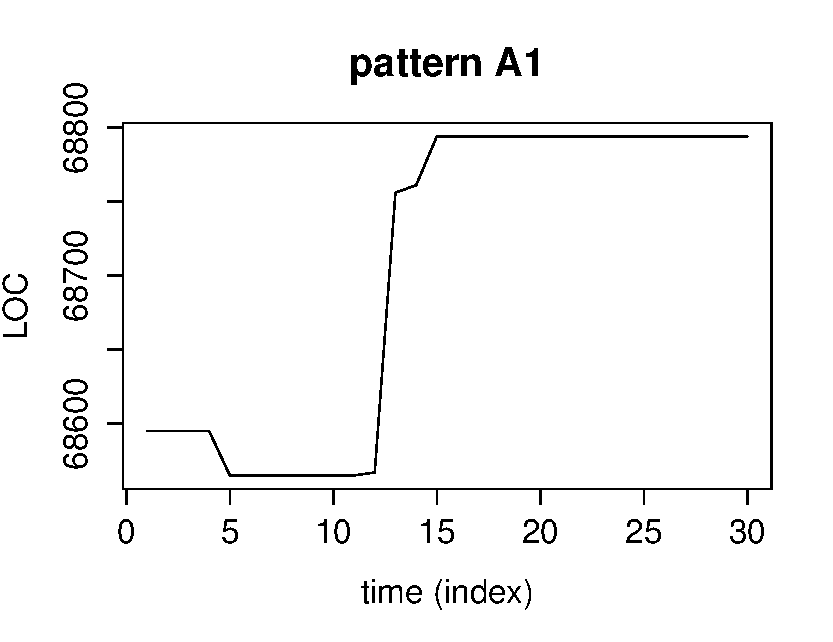
\includegraphics[width=196pt]{images/pattern_a1.pdf}
	\hspace{1em}
	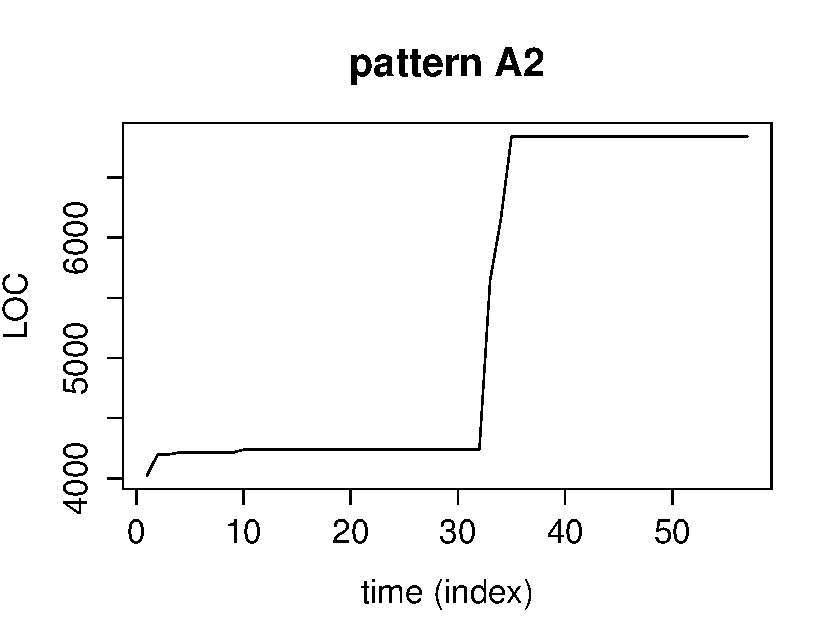
\includegraphics[width=196pt]{images/pattern_a2.pdf}
	\\
	\vspace{1em}
	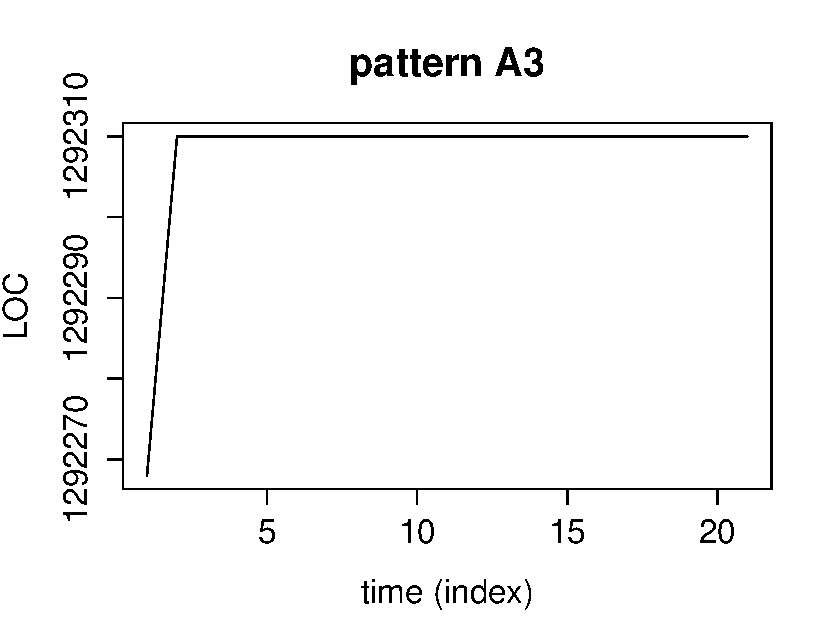
\includegraphics[width=196pt]{images/pattern_a3.pdf}
	\hspace{1em}
	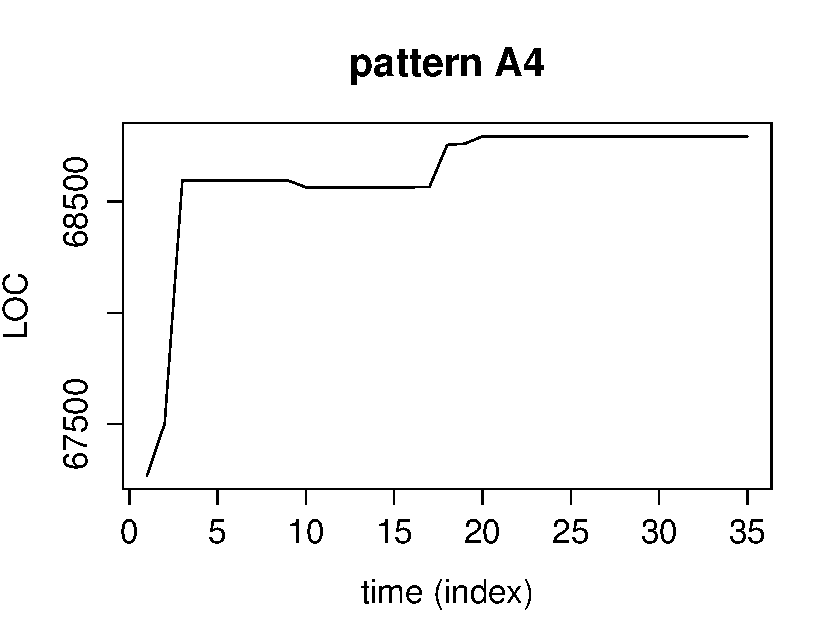
\includegraphics[width=196pt]{images/pattern_a4.pdf}
\end{figure}

\begin{comment}
- Factual results
- Tables and figures for clarification

This chapter presents and clarifies the results obtained during the research.
The focus should be on the factual results, not the interpretation or
discussion. Tables and graphics should be used to increase the clarity of the
results where applicable.
Have a look at the the results chapter in this example thesis on Paul’s
homepage\footnote{http://homepages.cwi.nl/~paulk/thesesMasterSoftwareEngineering/2006/ArnoldLankamp.pdf}.
\end{comment}
